%\documentclass[aps,prb,twocolumn,superscriptaddress,preprintnumbers,amsmath,amssymb,floatfix]{revtex4}
\documentclass[aps,prb,preprint,superscriptaddress,amsmath,amssymb,floatfix]{revtex4}
%\documentclass[aps,prl,onecolumn,groupedaddress,amsmath,amssymb,12pt]{revtex4}
\usepackage{graphicx}
\usepackage{ifthen}
\usepackage{dcolumn}% Align table columns on decimal point
\usepackage{bm}% bold math
\usepackage{multirow}
\usepackage{booktabs}
\usepackage{bm}% bold math
\usepackage{amsbsy}
\usepackage{amsmath}
\usepackage{amssymb}
\usepackage{subfigure}


%Definition of new commands
\newcommand{\f}[2]{\ensuremath{\frac{\displaystyle{#1}}{\displaystyle{#2}}}}
\newcommand{\lr}[1]{\langle{#1}\rangle}
\newcommand{\colv}[2] {\left(\begin{array}{c} #1 \\ #2 \end{array}\right)}
\renewcommand{\thefootnote}{\fnsymbol{footnote}}
\newcommand{\be} {\begin{eqnarray}}
\newcommand{\ee} {\end{eqnarray}}
%--------------------------------------------------------------------------
%EQ COMMANDS
%--------------------------------------------------------------------------
\newcommand{\two}{\mspace{-2.0mu}}
\newcommand{\four}{\mspace{-4.0mu}}
\newcommand{\plus}{\mspace{-4.5mu}+\mspace{-3.5mu}}
\newcommand{\minus}{\mspace{-4.5mu}-\mspace{-3.5mu}}
\newcommand{\pp}{'\mspace{-2.0mu}'}
\newcommand{\xlb}[4]{#1\ifthenelse{\equal{#2}{0}}{}{_{\alpha #2}}
\mspace{-2.0mu}\genfrac{(}{)}{0pt}{1}{\ifthenelse{\equal{#3}{0}}{0}{l #3}} 
{\ifthenelse{\equal{#4}{0}}{0}{b #4}}}

\newcommand{\xkv}[4]{#1\mspace{-5.0mu}\left(\mspace{-8.0mu}
\begin{smallmatrix}#2\four{}\four{}\mspace{-8.0mu}&\pmb{\kappa}#3\\&\nu 
#4\end{smallmatrix}\mspace{-5.0mu}\right)}

\newcommand{\evect}[6]{#1\mspace{-4.0mu}\left(\mspace{-8.0mu}
\begin{smallmatrix}#2\mspace{-8.0mu}&\pmb{\kappa} #3 &b #5\\&\nu #4 &
\alpha #6\end{smallmatrix}\mspace{-5.0mu}\right)}

\newcommand{\varmat}[8]{\mspace{-5.0mu}\left(\mspace{-8.0mu}
\begin{smallmatrix}\ifthenelse{\equal{#3}{0}}{\mspace{-8.0mu}&b_{#1}&b_{#2}
\\&\alpha_{#1}&\alpha_{#2}} {\ifthenelse{\equal{#7}{0}}{#1\mspace{-8.0mu}&
\pmb{\kappa}#2#3\mspace{-8.0mu}&\pmb{\kappa}#4#5\mspace{-8.0mu}&\pmb{\kappa}
#6\\&\nu#2&\nu#4&\nu#6} {#1\mspace{-8.0mu}&\pmb{\kappa}#2#3\mspace{-8.0mu}&
\pmb{\kappa}#4#5\mspace{-8.0mu}&\pmb{\kappa}#6#7\mspace{-8.0mu}&\pmb{\kappa}
#8\\&\nu#2&\nu#4&\nu#6&\nu#8}}\end{smallmatrix}\mspace{-5.0mu}\right)}

\newcommand{\EXP}[1]{\exp\mspace{-5.0mu}\left[#1\right]\mspace{-3.0mu}}

\newcommand{\tpp}[2]{\left(\mspace{-2.0mu}\xkv{\omega}{}{}{}#1\xkv{\omega}
{}{'}{'}#2\xkv{\omega}{}{\pp}{\pp}\mspace{-2.0mu}\right)}



%--------------------------------------------------------------------------
\newcommand{\SUM}[2]{\ifthenelse{\equal{#1}{0}}{\sum_{
\alpha_{#2},b_{#2},l_{#2}}^{3,n,N}} {\ifthenelse{\equal{#1}{1}}{\sum_{
\alpha_{#2},b_{#2}}^{3,n}}{\sum_{\pmb{\kappa}#2,\nu#2}^{N,3n}}}}

\newcommand{\SUMprime}[2]{\ifthenelse{\equal{#1}{0}}
{\sum_{\alpha_{#2},b_{#2},l_{#2}}^{3,n,N}} 
{\ifthenelse{\equal{#1}{1}}{\sum_{\alpha_{#2},b_{#2}}^{3,n}}
{\sum_{\pmb{\kappa}^{'}#2,\nu#2}^{N,3n}}}}

\newcommand{\SUMalpha}[2]{\ifthenelse{\equal{#1}{0}}
{\sum_{\alpha_{#2}}^{3}} {\ifthenelse{\equal{#1}{1}}
{\sum_{\alpha_{#2},b_{#2}}^{3,n}}{\sum_{\pmb{\kappa}#2,\nu#2}^{N,3n}}}}
%--------------------------------------------------------------------------
\newcommand{\SUMalphap}[2]{\ifthenelse{\equal{#1}{0}}
{\sum_{\alpha'_{#2}}^{3}} {\ifthenelse{\equal{#1}{1}}
{\sum_{\alpha'_{#2},b'_{#2}}^{3,n}}{\sum_{\pmb{\kappa}#2,\nu#2}^{N,3n}}}}

\newcommand{\SUMb}[2]{\ifthenelse{\equal{#1}{0}}{\sum_{b_{#2}}^{n}}
 {\ifthenelse{\equal{#1}{1}}{\sum_{\alpha_{#2},b_{#2}}^{3,n}}
{\sum_{\pmb{\kappa}#2,\nu#2}^{N,3n}}}}

\newcommand{\SUMbp}[2]{\ifthenelse{\equal{#1}{0}}{\sum_{b'_{#2}}^{n}}
 {\ifthenelse{\equal{#1}{1}}{\sum_{\alpha'_{#2},b'_{#2}}^{3,n}}
{\sum_{\pmb{\kappa}#2,\nu#2}^{N,3n}}}}

\newcommand{\SUMl}[2]{\ifthenelse{\equal{#1}{0}}{\sum_{l_{#2}}^{N}}
 {\ifthenelse{\equal{#1}{1}}{\sum_{\alpha_{#2},b_{#2}}^{3,n}}
{\sum_{\pmb{\kappa}#2,\nu#2}^{N,3n}}}}

\newcommand{\SUMlp}[2]{\ifthenelse{\equal{#1}{0}}{\sum_{l'_{#2}}^{N}}
 {\ifthenelse{\equal{#1}{1}}{\sum_{\alpha'_{#2},b'_{#2}}^{3,n}}
{\sum_{\pmb{\kappa}#2,\nu#2}^{N,3n}}}}

\newcommand{\abcdt}[5]{\mspace{-4.0mu}\left(\mspace{-8.0mu}
\begin{smallmatrix}&\ifthenelse{\equal{#1}{}}{a}{#1}&\ifthenelse
{\equal{#3}{}}{c}{#3}\\&\ifthenelse{\equal{#2}{}}{b}{#2}&\ifthenelse
{\equal{#4}{}}{d}{#4}\end{smallmatrix}\mspace{-2.0mu};\ifthenelse
{\equal{#5}{}}{t}{#5}\right)}

\newcommand{\abcd}[4]{\mspace{-4.0mu}\left(\mspace{-8.0mu}
\begin{smallmatrix}&\ifthenelse{\equal{#1}{}}{a}{#1}&\ifthenelse
{\equal{#3}{}}{c}{#3}\\&\ifthenelse{\equal{#2}{}}{b}{#2}&\ifthenelse
{\equal{#4}{}}{d}{#4}\end{smallmatrix}\mspace{-3.0mu}\right)}

\newcommand{\abt}[3]{\mspace{-4.0mu}\left(\mspace{-8.0mu}\begin
{smallmatrix}&\ifthenelse{\equal{#1}{}}{a}{#1} \\&\ifthenelse{
\equal{#2}{}}{b}{#2}\end{smallmatrix}\mspace{-2.0mu};
\ifthenelse{\equal{#3}{}}{t}{#3}\right)}

\newcommand{\ab}[2]{\mspace{-4.0mu}\left(\mspace{-8.0mu}
\begin{smallmatrix}&\ifthenelse{\equal{#1}{}}{a}{#1} \\&\ifthenelse
{\equal{#2}{}}{b}{#2}\end{smallmatrix}\mspace{-3.0mu}\right)}

\newcommand{\kvbat}{\mspace{-4.0mu}\left(\mspace{-8.0mu}
\begin{smallmatrix} &\pmb{\kappa} &b \\ &\nu &\alpha\end{smallmatrix}
\mspace{-2.0mu};t\right)}
%--------------------------------------------------------------------------
\newcommand{\kvbatp}{\mspace{-4.0mu}\left(\mspace{-8.0mu}
\begin{smallmatrix} &\pmb{\kappa} &b' \\ &\nu &\alpha'\end{smallmatrix}
\mspace{-2.0mu};t\right)}

\newcommand{\kvbaw}{\mspace{-4.0mu}\left(\mspace{-8.0mu}
\begin{smallmatrix} &\pmb{\kappa} &b \\ &\nu &\alpha\end{smallmatrix}
\mspace{-2.0mu};\omega\right)}

\newcommand{\kvbawp}{\mspace{-4.0mu}\left(\mspace{-8.0mu}
\begin{smallmatrix} &\pmb{\kappa} &b' \\ &\nu &\alpha'\end{smallmatrix}
\mspace{-2.0mu};\omega\right)}

\newcommand{\kvba}{\mspace{-4.0mu}\left(\mspace{-8.0mu}
\begin{smallmatrix} &\pmb{\kappa} &b \\ &\nu &\alpha\end{smallmatrix}
\mspace{-3.0mu}\right)}

\newcommand{\kvbap}{\mspace{-4.0mu}\left(\mspace{-8.0mu}
\begin{smallmatrix} &\pmb{\kappa} &b' \\ &\nu &\alpha'\end{smallmatrix}
\mspace{-3.0mu}\right)}
%--------------------------------------------------------------------------
\newcommand{\kpvba}{\mspace{-4.0mu}\left(\mspace{-8.0mu}
\begin{smallmatrix} &\pmb{\kappa}^{'} &b \\ &\nu &\alpha\end{smallmatrix}
\mspace{-3.0mu}\right)}

\newcommand{\kva}{\mspace{-4.0mu}\left(\mspace{-8.0mu}
\begin{smallmatrix} &\pmb{\kappa} \\ &\nu &\alpha\end{smallmatrix}
\mspace{-3.0mu}\right)}

\newcommand{\kvap}{\mspace{-4.0mu}\left(\mspace{-8.0mu}
\begin{smallmatrix} &\pmb{\kappa} \\ &\nu &\alpha'\end{smallmatrix}
\mspace{-3.0mu}\right)}

\newcommand{\kvb}{\mspace{-4.0mu}\left(\mspace{-8.0mu}
\begin{smallmatrix} &\pmb{\kappa} &b \\ &\nu \end{smallmatrix}
\mspace{-3.0mu}\right)}

\newcommand{\kvbp}{\mspace{-4.0mu}\left(\mspace{-8.0mu}
\begin{smallmatrix} &\pmb{\kappa} &b' \\ &\nu \end{smallmatrix}
\mspace{-3.0mu}\right)}

\newcommand{\kvt}{\mspace{-4.0mu}\left(\mspace{-8.0mu}
\begin{smallmatrix}&\pmb{\kappa} \\&\nu\end{smallmatrix}
\mspace{-2.0mu};t\right)}

\newcommand{\kpvt}{\mspace{-4.0mu}\left(\mspace{-8.0mu}
\begin{smallmatrix}&\pmb{\kappa}^{'} \\&\nu\end{smallmatrix}
\mspace{-2.0mu};t\right)}

\newcommand{\kvw}{\mspace{-4.0mu}\left(\mspace{-8.0mu}
\begin{smallmatrix}&\pmb{\kappa} \\&\nu\end{smallmatrix}
\mspace{-2.0mu};\omega\right)}

\newcommand{\kv}{\mspace{-4.0mu}\left(\mspace{-8.0mu}
\begin{smallmatrix}&\pmb{\kappa} \\&\nu\end{smallmatrix}
\mspace{-3.0mu}\right)}

\newcommand{\kpvp}{\mspace{-4.0mu}\left(\mspace{-8.0mu}
\begin{smallmatrix}&\pmb{\kappa'} \\&\nu'\end{smallmatrix}
\mspace{-3.0mu}\right)}
%--------------------------------------------------------------------------
\newcommand{\lbt}{\mspace{-4.0mu}\left(\mspace{-8.0mu}
\begin{smallmatrix}&l \\&b\end{smallmatrix}\mspace{-2.0mu};t\right)}

\newcommand{\lbtp}{\mspace{-4.0mu}\left(\mspace{-8.0mu}
\begin{smallmatrix}&l' \\&b'\end{smallmatrix}\mspace{-2.0mu};t\right)}

\newcommand{\lt}{\mspace{-4.0mu}\left(\mspace{-8.0mu}
\begin{smallmatrix}&l\end{smallmatrix}\mspace{-2.0mu};t\right)}

\newcommand{\ltp}{\mspace{-4.0mu}\left(\mspace{-8.0mu}
\begin{smallmatrix}&l'\end{smallmatrix}\mspace{-2.0mu};t\right)}

\newcommand{\lb}{\mspace{-4.0mu}\left(\mspace{-8.0mu}
\begin{smallmatrix}&l \\&b\end{smallmatrix}\mspace{-3.0mu}\right)}

\newcommand{\lbp}{\mspace{-4.0mu}\left(\mspace{-8.0mu}
\begin{smallmatrix}&l' \\&b'\end{smallmatrix}\mspace{-3.0mu}\right)}
%--------------------------------------------------------------------------
%COMMANDS
%--------------------------------------------------------------------------

\begin{document}


\title{Predicting Vibrational Mean Free Paths in Disordered Systems}

\author{Jason M. Larkin}
\affiliation{Department of Mechanical Engineering\\Carnegie Mellon 
University\\Pittsburgh, PA 15213}
\author{Joseph E. Turney}
\affiliation{Department of Mechanical Engineering\\Carnegie Mellon 
University\\Pittsburgh, PA 15213}
\author{Alexandre D. Massicotte}
\affiliation{Department of Mechanical Engineering\\Carnegie Mellon 
University\\Pittsburgh, PA 15213}
\author{Cristina H. Amon}
\affiliation{Department of Mechanical Engineering\\Carnegie Mellon 
University\\Pittsburgh, PA 15213}
\affiliation{
Department of Mechanical \& Industrial Engineering, University of Toronto,
Toronto, Ontario, Canada M5S 3G8}
\author{A. J. H. McGaughey}
\email{mcgaughey@cmu.edu}
\affiliation{Department of Mechanical Engineering\\
Carnegie Mellon University\\Pittsburgh, PA 15213}

%--------------------------------------------------------------------------

\date{\today}

\begin{abstract}

\end{abstract}


\maketitle
%--------------------------------------------------------------------------
\clearpage
\section{\label{S:Introduction}Introduction}
%--------------------------------------------------------------------------
The thermal conductivity of amorphous solids display 
unique temperature dependance compared to ordered solids.
\cite{freeman_thermal_1986}

Measurements by all the refs from Galli paper, including Moon.
\cite{wada_thermal_1996}\cite{zink_thermal_2006}
\cite{yang_anomalously_2010}\cite{cahill_thermal_1994}
\cite{kuo_thermal_1992}\cite{moon_thermal_2002}
\cite{liu_high_2009}

The key to understanding such measurement is to estimate a MFP for the 
vibrational modes in disordered systems. 

Cahill argued that the lattice vibrations in a disordered crystal are 
essentially the same as those of an amorhous solid.
\cite{cahill_lower_1992} 

The goal of this work is to predict the MFP of vibrational modes in 
disordered systems. Simple Lennard-Jones systems will be studied.  A 
perfect LJ crystal are alloyed with a species of differing mass and 
amorphous samples are prepared. The vibrational modes in these systems are
characterized in the limit of propagating (phonon) and 
non-propagating (diffuson) modes by predicting the mode lifetimes and 
estimating their mean free paths. Estimating an effective dispersion
relation is necessary for calculating an effective group velocity for 
disordered, which is crucial for transforming lifetimes to MFPs.
The spectrum of phonon MFPs and the accumulated thermal conductivity 
are predicted for a model of amorphous silicon. Predictions of thermal 
conductivity using a boundary scattering model demonstrates  

Ref Cahill paper, vg=vs. Ref Galli paper, its unclear what the group 
velocity should be.\cite{he_heat_2011}



\section{\label{S:Lifetimes}Thermal Conductivity Predictions for 
Disordered Solids from Molecular Dynamics}
%--------------------------------------------------------------------------
The thermal conductivity of amorphous solids at low temperatures contain 
quantum statistical effects.\cite{freeman_thermal_1986} Molecular dynamics 
simulations are not able to capture quantum statistical effects.

Plot GK results for LJ crystal-alloy-amor


\section{\label{S:Lifetimes}Kinetic Theory}
%--------------------------------------------------------------------------

k = sum over modes

For a perfect system, all vibrational modes are phonons.  It is thus easy 
to evaluate.

Diffusons, locons and propagons \cite{allen_diffusons_1999}.

\section{\label{S:Lifetimes}Lifetimes of Disordered Modes}
%--------------------------------------------------------------------------

Lifetimes in amorphous silicon predicted before using a normal mode 
approach, but mode-by-mode properties were not presented.
 \cite{bickham_calculation_1998}

Lifetimes were predicted using anharmonic lattice dynamics, but no thermal 
transport properties were predicted.\cite{fabian_anharmonic_1996}

Thermal diffusivity was predicted for a percolation network which showed 
Rayleigh type scattering dependance in the low-frequency limit.
\cite{sheng_heat_1991}

Thermal diffusivity has been predicted using a wave-packet method

The lifetimes of vibrational modes in a-Si were predicted using normal 
mode decomposition.\cite{he_heat_2011}

\subsection{\label{S:Lifetimes:}Ioffe-Regel Limit}
%--------------------------------------------------------------------------



\section{\label{S:Lifetimes}Thermal Conductivity Diffusivity}
%--------------------------------------------------------------------------


In this work, we predict the lifetimes of vibrational modes using normal 
mode decomposition \cite{turney_predicting_2009-1}.


Previous studies \cite{he_heat_2011}.

\section{\label{S-Motivation}Allen Feldman Diffusivity}
%--------------------------------------------------------------------------

Allen Feldman theory \cite{allen_thermal_1993}.

Feldman measure the DOS using the average level spacing.
\cite{feldman_numerical_1999} 

Predictions for a-Si, also effects of mass disorder.
\cite{feldman_thermal_1993}: is Di pinned near a value of Di~(1/3)va?

\subsection{\label{S-Motivation-Amorphous}Limits of the AF Diffusivity}
%--------------------------------------------------------------------------
It was noticed by Birch and Clark (1940), and by Kit-
tel (1948) that in glasses κ(T ) at T >20K could be in-
terpreted as the specific heat C(T )/V multiplied by a
 ̄
temperature-independent diffusivity D of order a2 ωD /3
where a is an interatomic distance. In the phonon-gas
model, this would correspond to l ≈ a, too small to jus-
tify use of the model. The success of this observation
implies that the dominant normal modes in a glass are of
the D variety, not P because P implies l ≫ a, and not L
because L implies D = 0 until anharmonic corrections are
added which make D depend on T . This successful (and
we believe, essentially correct) interpretation lost favor
after Anderson localization was understood, because a
misconception arose that the P/D boundary (which cer-
tainly lies low in the spectrum of a glass) should lie close
to the E/L boundary.

Limits of D(w)

/home/jason/Downloads/papers/disorder/PhysRevB.43.6573.pdf
/home/jason/Downloads/papers/disorder/9907132.pdf


\subsection{\label{S:Lifetimes:}Characterization of Vibrational Modes}
%--------------------------------------------------------------------------
If determined by the Ioffe-Regel limit, $\tau \kv < 1/\omega \kv$.
\cite{taraskin_determination_1999} However, for thermal transport 
analysis this definition is not useful on its own. Show that Anderson 
loclization is exponetial depenance of mode excitation on distance from 
some local center\cite{feldman_numerical_1999}. If Ioffe-Regel limit is 

According to Cahill, the lifetimes of vibrations in amorphous materials 
is taken to be one half the period, $\tau = \pi/\omega $.
\cite{cahill_heat_1989}

The dynamic structure factor can be useful for demonstrating the 
plane-wave character of low-frequency vibrations.  However, on a 
mode-by-mode basis, it is unable in general to characterize a given mode 
as either localized or delocalized.  In fact, results   
frequency modes in a disordered systems

Participation ratio:
For a finite system, the participation is limited by system size.
evolution of a vibrational wave packet on a disordered chain.
\cite{allen_evolution_1998}, shows participation ratio limitation. Also 
\cite{garber_numerical_2001}.


\subsection{\label{S:Lifetimes:}Localization of Disordered Modes}
%--------------------------------------------------------------------------
Modes can







\subsection{\label{S:Lifetimes:}Normal Mode Decomposition}
%--------------------------------------------------------------------------
Normal mode decomposition and its limitations.
\cite{turney_predicting_2009-1} 

If $\gamma \kv > \omega \kv$, then the vibrational mode is overdamped.  
Discuss why real-space method is necessary in this case.





\section{\label{S:GroupVeloctiy}Effective Mode Velocity}

\subsection{\label{S:Lifetimes:}Dynamic Structrue Factor}

If all modes are summed over, this gives the frequency spectrum
needed to construct a (nonstationary) propagating state with a
pure wave vector Q and pure longitudinal or transverse polarization
 \cite{feldman_thermal_1993}. Locations of spectral peaks are peaked 
like a acoustic dispersion branches. Only low-frequency vibrations 
have an (approximate) wavevector in disordered systems, and there is 
no theorem guranteeing this. \cite{feldman_numerical_1999}

However, it is very
difficult to distinguish between localized and extended
modes at high frequencies on the basis of their f(k, ro)
functions, as illustrated by the very similar scattering
functions for a 67-meV localized and a 63-meV extended
mode in Fig. 3(b). \cite{biswas_vibrational_1988}


\section{\label{S-Motivation}Characterization}
%--------------------------------------------------------------------------

Determine by mean free path condition:

$\Lambda > \lambda$

Requires a 

\section{\label{S-Motivation}Effective Velocities of Vibrational Modes}
%--------------------------------------------------------------------------




It is difficult to assign a wavevector (and hence a wavelength) to 
disordered mode.  Therefore, some limit must be imposed:

$\Lambda > a$

Where a is the lattice spacing.

\section{\label{S-Motivation}Ordered Alloys}
%--------------------------------------------------------------------------

\subsection{\label{S-Introduction-OrderedAlloy-PhonoDispersion}Phonon 
Dispersion}
%--------------------------------------------------------------------------
- $v_g(m_{r})$

- two masses with $v_g(m_{r})$, maybe compare with 4 masses with higher mass 
ratio.  

- Keep  $m_{avg}$ constant for all.

- run a system with a "softer" and "stiffer" LJ (smaller/bigger eps or sigma). 
This can be used as a comparison for the phonon/diffuson spectrums which will be 
shown later.  


\subsection{\label{S-Introduction-OrderedAlloy-PhonoLife}Phonon Lifetimes}

- compare lifetimes from 2 atom alloy, 4 atom alloy.  Is the reduction in thermal conductivity mostly due to the reduction in group velocities/introduction of optical modes?


\section{\label{S-Motivation}Disordered Alloys}

\subsection{\label{S-Motivation-Amorphous}Effective Phonon Dispersion}

- compare versus virtual crystal

\subsection{\label{S-Motivation-Amorphous}Effective Phonon Lifetimes}

- compare c=0.0,0.05,0.15

- why not bond disorder?  This has been investigated such as in Schelling Si/Ge \cite{schelling2002}, Marzari Si/Ge PRL \cite{Garg2011}.  Although, detailed study of PbTe/PbSe systems (Esfarjani/Shiomi preprint) demonstrate the importance of bond environment for alloys.

- if consider bond disorder, pick a "softer/stiffer" system. This system should be less/more sensitive to alloying which is discussed later.  Could reference the PbTe/PbSe paper about this.

- compare these predicted lifetimes to predictions from:

\begin{equation}\label{EQ:M:ZT}
\begin{split}
\frac{1}{\tau_{mass}} = \frac{\pi}{2N}\omega^2\kv \sum_{\pmb{\kappa'},\nu'}^{N,3n} \delta(\omega\kv - \omega\kpvp) \sum_{b}^{n}g(b)|e^*\kvba \dot e\kvba|^2 , \\
\end{split}
\end{equation}

$g(b) = \sum_{i} f_i(b)[1-m_i(b)/m_{avg}(b)]^2$

\subsection{\label{S-Motivation-Amorphous}Disappearance of SED Peaks}

- show SED plot of mode peaks from c=0.0,0.05,0.15,0.5 for any mode where a peak still shows in 0.5

\subsection{\label{S-Motivation-Amorphous}Propagating Modes in Heavily Disordered Alloys}

- Analysis of c=0.5 modes at gamma, which modes are plane-wave like? 


\section{\label{S-Motivation} Heat Transport in Amorphous System}

\subsection{\label{S-Motivation-Amorphous}Effective Phonon Dispersion}

- compare predicted sound speeds from finite dispersion acoustic branch (dk~pi/100L), bulk modulus

\subsection{\label{S-Motivation-Amorphous}Allen Feldman Diffuson Theory}

- thermal transport in terms of a diffusivity, no need for a propagation velocity

\subsection{\label{S-Motivation-Amorphous}Diffuson Lifetimes}

- measured using NMD and anharmonic MD.

- extract effective Diffuson velocity, compare to sound speed

- use sound speed to predict a phonon MFP, establish a MFP cut-off criteria to call something a phonon or not.  Could be MFP > lattice constant or something.  However, there are no wavelengths (yet).

\subsection{\label{S-Motivation-Amorphous}Propagating Modes in Amorphous System}

- Analysis of c=0.5 modes at gamma, which modes are plane-wave like? This will be the key to the length scale needed to compare with the MFP predicted above. The plane-wave like modes will be identified by fourier transforming the eigvec.  It should show content at a small number of wavevectors, and 1 should be dominant and of the order of pi/L. 

\subsection{\label{S-Motivation-Amorphous}Role of Anharmonicity in Disordered Thermal Transport}

- run harmoninc FC MD, predict thermal conductivity using GK

- compare anharmonic GK, harmonic GK, and AF predictions. May possibly need to run "stiffer" system to compare with $k_{si} = k_{ph} + k{AF} = 0.5+0.5$. 

\section{\label{S-Motivation} Thermal Diffusivity in Ordered and Disordered Systems}



- plot AF and phonon diffusivities for all systems above.  

- Show that for high mass ratio ordered alloys and disordered alloys, the thermal diffusivities are on the order of amorphous system. 

- For high mass ratio ordered alloys, it is the reduction of the group velocities through decreased acoustic and introduced optical branches. 

- For the disordered alloys, the phonon lifetimes of high frequency modes are drastically reduced as alloy concentration is increased.  Should show that this effect is less drastic for "soft" (soft bond) or "acoustically" matched systems (low mass ratio). It is more drastic for large acoustically mismatched systems (high mass ratio) or stiff systems.

- For amorphous systems, there is not a unique choice of the phonon MFP. Instead, it is helpful to consider the diffusons and their thermal diffusitivty. Compared to high mass ratio ordered alloys and heavily disordered alloys, these thermal diffusivities are comparable.  

- Compare high mass ratio ordered alloys optical branch group velocities/lifetimes (diffusivities) to amorphous diffusivities ("group velocity" and "lifetime"). Are they really distinguishable?











\appendix
\section{\label{A-Predicting-Phonons}Predicting Phonon Properties}
\subsection{\label{A-Phonon-Normal-Modes}Vibrations in Ordered and Disordered Solids}
In a crystal (periodic) system, the vibrations of atoms are described by a basis of eigenfunctions called phonon normal modes, which are determined by the properties of the crystal (see Appendix \ref{A-Allowed-Wavevectors-Ordered}). The eigenvalues of this basis are the phonon mode frequencies (energies).\cite{dove1993,wallace1972} The atomic velocities can be represented by the velocity normal mode coordinate, defined as 
\cite{dove1993}
\begin{equation}\label{E:udot_HLD}
\begin{split}
\dot{u}_{\alpha}\lbt = &\SUMprime{2}{} \frac{1}{\sqrt{m_bN}} \EXP{i\pmb{\kappa}^{'}\cdot\mathbf{r}_0\ab{l}{0}} e^*\kvba \dot{q}\kvt{}{}{}.
\end{split}
\end{equation}
Here, $\dot{q}\kvt{}{}{}$ represents the kinetic energy $T \kvt$ of the mode with phonon frequency $\omega_0\kv$ by
\cite{dove1993}
\begin{equation}\label{E:udot_HLD}
\begin{split}
T \kvt= \frac{\dot{q}^*\kvt{}{}{}\dot{q}\kvt{}{}{}}{2}.
\end{split}
\end{equation}
The phonon mode kinetic energies $T \kvt$ are used to calculate the phonon spectral energy denisty in Appendix \ref{A-Phonon-Life-SED}.
\subsection{\label{A-Phonon-Life-SED}Predicting Phonon Lifetimes using Spectral Energy Denisty}
The phonon normal mode coordinate is,
\begin{equation}\label{EQ:NMD:qdot}
\begin{split}
\dot{q}\kvt{}{}{}=&\SUM{0}{}\sqrt{\frac{m_b}{N}}\dot{u}_{\alpha}\lbt e^*\kvba\EXP{i\pmb{\kappa}\cdot\mathbf{r}_0\ab{l}{0}},
\end{split}
\end{equation}
which form the basis for vibrations in ordered materials and represents the phonon mode kinetic energy. The normal mode kinetic energy can be transformed from the time domain $t$ to the
frequency domain $\omega$ by Parseval's theorem,\cite{rudin1987}
\begin{equation}\label{EQ:NMD:KE_single}
\begin{split}
T\kvw=&\lim_{\tau_0\rightarrow\infty}\frac{1}{2\tau_0}\left|\frac{1}{\sqrt{2\pi}}\int_{0}^{\tau_0}\dot{q}\kvt\exp(-i\omega t)dt\right|^2.
\end{split}
\end{equation}
Here, $T\kvw$ represents the spectral energy of the phonon normal mode with frequency $\omega\kvw$. Following the derivation in Appendix \ref{A-Derivation-SED}, one arrives at the expression for the SED of a single phonon mode,
\begin{equation}\label{E:Lorentzian_NMD_2}
\begin{split}
T\kvw = \frac{C_0\kv}{2}\frac{\Gamma\kv/\pi}{[\omega_0\kv-\omega]^2+\Gamma^2\kv},
\end{split}
\end{equation}
which is a Lorentzian function with center at $\omega_0\kv$ and a half-width at half-maximum (linewidth) of
$\Gamma\kv$ and $C_0\kv$ is a constant. We know from anharmonic lattice dynamics theory that the phonon linewidth is related to the phonon lifetime, $\tau\kv$, by\cite{maradudin1962,ladd1986}
\begin{equation}\label{E:lifetime}
\begin{split}
\tau\kv=&\frac{1}{2\Gamma\kv}.
\end{split}
\end{equation}
The MD simulations we perform here are classical. For a classical system in the harmonic limit (i.e., temperature approaching zero) there is an equipartition of energy and $\sum_{\nu}^{3n} T\kvw = \sum_{\nu}^{3n} V\kvw$.\cite{mcquarrie2000} In an anharmonic system (i.e., a MD simulation), the assumption of equipartition of energy can be tested by predicting the system-level specific heat. By assuming equipartition of energy, the phonon SED at a particular wavevector is
\begin{equation}\label{EQ:NMD-LorLorentzian_NMD}
\begin{split}
\Phi(\pmb{\kappa},\omega) = 2\sum_{\nu}^{3n} T\kvw =& \sum_{\nu}^{3n}C_0\kv\frac{\Gamma\kv/\pi}{[\omega_0\kv-\omega]^2+\Gamma^2\kv},
\end{split}
\end{equation}
which is a superposition of $3n$ Lorentzian functions with centers at $\omega_0\kv$ (one for each polarization). For simplicity, we refer to $\Phi(\pmb{\kappa},\omega)$ as $\Phi$. Given a set of atomic velocities, $\Phi$ can be calculated using Eq$.$ \eqref{E:qdot_HLD} and \eqref{A:E:ave_T_w1}, and then fit using Eq$.$ \eqref{A:E:Lorentzian_NMD} to extract the phonon properties $\omega_0\kv$ and $\tau\kv$.
\begin{figure}
\begin{center}
%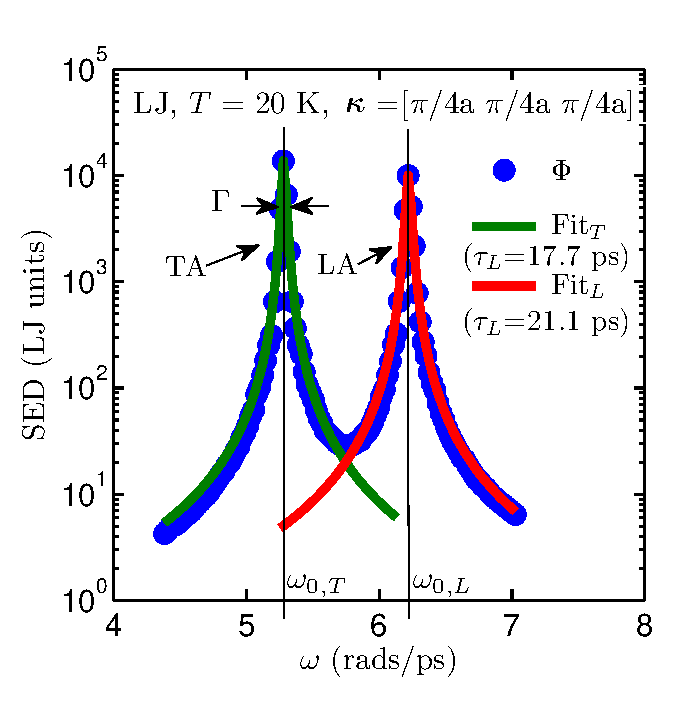
\includegraphics[angle=0,width=70.0mm]{lj_fit_peak.eps}
\vspace*{-5mm}
\end{center}
\caption{\label{FIG:LJ_FIT_PEAK} The SED ($\Phi$) for the first three polarizations at the wavevector $[\pi/4a,\pi/4a,\pi/4a]$ for LJ argon at a temperature of 20 K. There are two degenerate transverse acoustic polarizations and one longitudinal acoustic polarization (of higher frequency).\cite{dove1993} When fitting the SED, the different polarizations can be fit individually using single Lorentzian peaks or as a superposition of peaks. Here the two peaks are fit individually with $\Phi$ plotted as a superposition. The predicted lifetimes of these polarizations, which are inversely proportional to the peak widths $\Gamma$, are provided in the legend.}
\end{figure}

\subsection{\label{A-Allowed-Wavevectors-Ordered}Allowed Wavevectors in Ordered Systems}
The phonon spectral energy is defined for the allowed wavevectors of a crystal, which can be specified from the crystal structure's Bravais lattice and its basis, i.e. unit cell. A $D$-dimensional Bravais lattice is a collection of points with
positions
\begin{equation}\label{crys_pos}
\begin{split}
\mathbf{u}_0\ab{l}{0} =& \sum^D_{\alpha} N_{\alpha}\mathbf{a}_{\alpha}
\end{split}
\end{equation}
where $N_{\alpha}$ and the summations if over the lattice vectors, $\mathbf{a}_{\alpha}$.\cite{ashcroft1976} The basis (or unit cell) is the building block of the crystal and they are arranged on the points defined by the Bravais lattice. The equillibrium position of any atom in the crystal can be described by
\begin{equation}\label{crys_pos2}
\begin{split}
\mathbf{u}_0\ab{l}{b} = \mathbf{u}_0\ab{l}{0} + \mathbf{u}_0\ab{0}{b}
\end{split}
\end{equation}
where $\mathbf{u}_0\ab{l}{0}$ is the equilibrium position of the $l^{\textrm{th}}$ unit cell and $\mathbf{u}_0\ab{0}{b}$ is the equilibrium position of the and $b^{\textrm{th}}$ atom in the unit cell relative to $\mathbf{u}_0\ab{l}{0}$.
For the LJ systems studied here, the cubic conventional cells are used with four atoms per unit cell.\cite{ashcroft1976} For our MD simulations, cubic simulation domains with periodic boundary conditions are used with $N_1 = N_2 = N_3 = N_0$.\cite{turney2009a,mcgaughey2004a} The allowed wavevectors for such crystal structures are
\begin{equation}\label{crys_pos3}
\begin{split}
\pmb{\kappa} = \sum_{\alpha} \mathbf{b}_{\alpha} \frac{n_{\alpha}}{N_{\alpha}},
\end{split}
\end{equation}
where $\mathbf{b}_{\alpha}$ are the reciprocal lattice vectors\cite{ashcroft1976} and $-N_{\alpha}/2 < n_{\alpha} \leq N_{\alpha}/2$, where $n_{\alpha}$ are integers and $N_{\alpha}$ are even integers.\cite{turney2009a} The wavevectors are taken to be in the first Brioullin zone.\cite{ashcroft1976}

\subsubsection*{Allowed Wavevectors in Disordered Materials}

Strictly speaking, the only allowed wavector in a disordered system is the gamma point ($\kappa = [0 0 0]$). As such, the lattice dynamics calculations are performed at the gamma point:


\subsection{\label{A-Thermal-Cond}Thermal Conductivity}
Once the lifetimes (MFPs) and group velocities of all virbrational modes in the
Brillouin zone are obtained, the bulk thermal conductivity in direction
$\mathbf{n}$, $k_{\mathbf{n}}$, can be calculated from \cite{ziman2001}
\begin{equation}\label{E-size:k_bulk}\
\begin{split}
k_{\mathbf{n}}=&\sum_{\pmb{\kappa}} \sum_\nu c_{ph} \kv v^{2}_{g,\mathbf{n}} \kv \tau \kv.
\end{split}
\end{equation}
Here, $c_{ph}$ is the phonon volumetric specific heat and ${v}_{g,\mathbf{n}}$ is
the component of the group velocity vector in direction $\mathbf{n}$. Since the systems we consider are classical and obey Maxwell-Boltzmann statistics,\cite{mcquarrie2000} the
specific heat is $k_{B}/V$ per mode in the harmonic limit where $V$ is the system volume. This approximation is used here and has been shown to be suitable for LJ argon\cite{mcgaughey2004c} and SW silicon.\cite{goicochea2010} The group
velocity vector is the gradient of the dispersion curves (i.e., $\partial \omega / \partial \pmb{\kappa}$), which can be calculated from the frequencies and wavevectors using finite differences. In this work, the group velocities are calculated using finite difference and quasi-harmonic lattice dynamics because a very small finite difference can be used which reduces the error.\cite{mcgaughey2006b} To predict a bulk thermal conductivity, it is necessary to perform a finite simulation size scaling procedure as discussed in Appendix \ref{A-Finite-Sim}.
\section{\label{A-Finite-Sim}Finite Simulation-Size Scaling for Thermal Conductivity}
For the LJ argon system studied in Section \ref{S-Prelim-Vib-Cond-Ordered}, a finite simulation-size scaling procedure\cite{turney2009a,He2011a} is used to compare the thermal conductivity predictions from $\Phi$ and $\Phi'$ to those from the Green-Kubo method. The scaling procedure is demonstrated in Fig$.$ \ref{FIG:LJ_COND}. The thermal conductivity is predicted from $\Phi$ or $\Phi'$ and MD simulations with $N_0 = 4,6,8,$ and $10$. The bulk conductivity, $k_{\infty}$, is then estimated by fitting the data to
\begin{equation}\label{k_size}
\begin{split}
1/k = 1/k_{\infty} + A/N_0,
\end{split}
\end{equation}
where $A$ is a constant. This procedure is necessary because the first Brillouin zone is only sampled at a finite number of points for a finite simulation size, with no contribution from the volume at its center. To predict a bulk thermal conductivity, it is important to sample points near the Brillouin zone center, where the modes can have large lifetimes and group velocities.\cite{turney2009a,sellan2010b} 
%This method has been validated for non-equilibrium MD simulations \cite{sellan2010a}, but has not been validated for equilibrium MD.
\begin{figure}
\begin{center}
%\includegraphics[angle=0,width=70.0mm]{LJ_NMD_SED_COND_2.eps}
\end{center}
\caption{\label{FIG:LJ_COND} Thermal conductivity predictions for LJ argon calculated using phonon lifetimes predicted by $\Phi$ and $\Phi'$.\cite{Larkin2012} (a) The finite simulation-size scaling extrapolation \cite{turney2009a,He2011a} is used to compare the results to bulk predictions made using the Green-Kubo method. (b) The bulk results for $\Phi$ and Green-Kubo are in good agreement temperatures of $20$ and $40$ K with those of other atomistic simulation methods.\cite{turney2009a}}
\end{figure}



\clearpage
\bibliographystyle{apsrev}
\bibliography{/home/jason/ntpl-ref/ntpl-jason/ntpl-jason-091412}
\end{document}
